\section{TRB Ring}

One of the primary means of communication with the HC, apart from register
interface, are the TRB rings. Their management is fully contained in the TRB
ring module. Before we dive into the implementation details, let us first
describe how these rings works.

\subsection{Architectural overview}

\emph{Transaction Request Block}, everywhere else abbreviated as TRB, is
a fixed-size structure with contents of variable type. The most notable
exception being a \emph{TRB Type} field. Each of the 64 TRB types defines the
other fields that are contained inside a TRB. Most commonly, it just contains
a pointer to another buffer together with the size of the buffer, or a result
of an operation.

\emph{TRB Ring} is then a circular queue comprised of individual TRBs. The main
difference from older HCIs is that TRBs are required to be contiguous in
memory, forming a \emph{TRB Ring Segment}. It is of course needed to link the
two ends of the segment together, one must use a special TRB type called
\emph{Link TRB}, which serves as a glue between the end and the beginning of
a segment. It is not required from the ring to be composed of only one segment,
but then special precautions must be taken.

TRB Ring is used in many instances during the lifetime of the Host Controller.
There are two special instances though: the \emph{Command Ring} and the
\emph{Event Ring}. The command ring serves as a channel to command the HC, and
the command interface is described in more depth in section \ref{sec:commands}.
The event ring is asynchronously read to retrieve results of commands,
completed transactions and so on, as the primary information channel from HC to
host. Actually, there can be more than one instance of Event Ring, but that
requires the host to be able to recognise multiple interrupts, which is not
supported in the current version of HelenOS. The event subsystem is further
discussed in the section \ref{sec:events}. The third type of a~ring,
a~\emph{Transfer Ring}, is used for every pipe endpoint on the bus - either
Endpoint or a Stream. These are used by the Transfer module, described in
section \ref{sec:transfers}. For now, let's discover the mechanics of the rings
themselves, regardless of their type.

As already said, TRB ring is a circular queue. It always has one producer and
one consumer of TRBs. Every ring implicitly defines two pointers: the enqueue
pointer and the dequeue pointer. The producer uses the enqueue pointer to
enqueue TRBs, and the consumer the dequeue pointer to dequeue ones. The
pointers are not shared between the host and the Host Controller. Instead,
every TRB have one bit with special semantics, the \emph{Cycle Bit}. The
transition between values of TRB Cycle Bit of individual TRBs defines the
value of Enqueue pointer. An example situation is shown on the figure
\ref{fig:ring-simple}.

\begin{figure}[h]
	\centering
	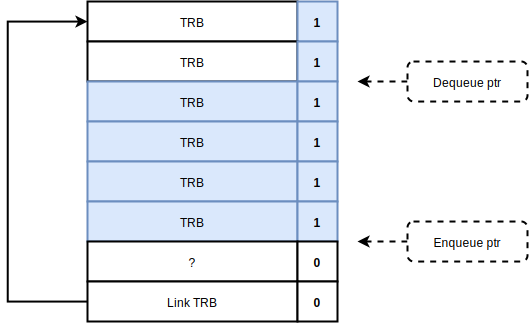
\includegraphics[width=0.6\textwidth]{ring-simple}
	\caption{A simple example of a TRB ring.}
	\label{fig:ring-simple}
\end{figure}

It is important to understand, that the consumer cannot write to the ring, and
thus cannot change the value of the Cycle Bit after it processes a TRB.
Therefore, the position of the dequeue pointer must be signalized by other
means. Furthermore, there has to be a mechanism to stop the consumer from
considering the TRBs in the beginning of the segment as enqueued, after it
wraps around the segment boundary. The enqueue pointer is not defined by
a transition from one to zero, but more generally by a transition from
\emph{Producer Cycle State}, \texttt{PCS} to \texttt{\textasciitilde PCS}.
This bit is kept in the memory of the producer. Similarly, there exists
a \emph{Consumer Cycle State}, which has the same value as \texttt{PCS} had in
the moment when the value of the enqueue pointer was the same as the current
value of the dequeue pointer.

The Link TRB contains a \emph{Toggle Cycle} flag, which if set, instructs both
producer and consumer to toggle its cycle state when this TRB is
enqueued/dequeued (Link TRBs are not necessarily fixed in place, they are queue
members as any other TRB). There shall always be an odd number of Link TRBs
with the Toggle Cycle flag set on the ring.

We haven't yet covered how the producer can be aware of the dequeue pointer
value. In case of Command and Transfer rings, the producer is the Host
Controller. Every finished command or transfer is denoted by an Event TRB
placed on the Event Ring. This Event TRB usually contains the physical address
of the TRB on the respective Command or Transfer ring. This way the producer
knows, that the dequeue pointer value is not less than the reported value.
Similarly, when the host processes an Event TRB on the Event Ring, it shall
report the physical address of the TRB processed by writing the value into
a dedicated register.

Also, the Event ring differs a bit in the usage of multiple segments. As the
Host Controller is obviously unable to allocate ring segments and map them into
virtual address space of the driver, and it's even not possible to allow the
host to write Link TRBs onto the ring, which is otherwise read-only for the
host, a~different approach has to be used. Instead of the segments being linked
together, the host preallocates a number of segments, and an \emph{Event Ring
Segment Table}, which is another structure defined by the specification. The
segments' addresses and sizes are written into the table, and the address of
the table is written to a dedicated register. At the time of the write, the
ownership of all the buffers is transferred to the Host Controller.

\subsection{Implementation}

As the requirements imposed by the specifications are quite strict, there's not
much freedom in the implementation. However, there were some decisions to be
discussed.

At first, we decided not to restrict ourselves on single-segment rings, as
other existing implementations do. We did not implemented runtime scaling of
the rings yet, though. Second, we implement and use three types of TRB rings;
the third one being a simplified TRB ring used by the host from both sides. Its
purpose is better described in the section \ref{sec:events}. The three
implementations are somehow separate, but because they share principles, they
reside in a common module.

The containing structures are called \struct{xhci_trb_ring_t},
\struct{xhci_event_ring_t} and \struct{xhci_sw_ring_t} for Command/Transfer
rings, Event ring and host-only rings, respectively. Despite their name, these
structures only represent the ring in host memory, and are not the structures
given to the hardware. Let's walk through them one by one.

\subsubsection{Command and Transfer Rings}

These rings are prepared to be multi-segment. They contain a list of
\struct{trb_segment_t} structures, which represent one ring segment. The
segment itself is allocated as a DMA buffer (sect. \ref{sec:dma-buffers}) of
size \macro{PAGE_SIZE}. The space for TRBs is in the beginning to ensure
alignment. At the end, there is a small footer keeping the physical address of
the segment and a link to the segment list. There are helper functions to
manage segments.

To avoid keeping the \struct{dma_buffer_t} structure inside the segment and
wasting precious DMA-accessible memory, the structure is reconstructed in order
to be freed in \fnc{trb_segment_free}. We agree that this violates the
encapsulation DMA buffers, but consider this the lesser evil.

The main runtime interface to rings of this kind is the method
\fnc{xhci_trb_ring_enqueue_multiple}, used to enqueue a contiguous array of
TRBs (referred to as Transfer Descriptor, TD) onto the ring. As this method
must not block to be usable in atomic contexts, it first performs a dry run to
check if there is enough space on the ring, then rollbacks and actually
emplaces the TRBs. Because it might be needed to interleave the Transfer
Descriptor with multiple Link TRBs, it is not possible to simply calculate the
free space in advance.

Because the caller of this function needs to know the physical address of the
TRB enqueued to pair it with the completion event, the address is assigned to
an output argument. If there are multiple TRBs to be enqueued, the one with
\emph{Interrupt On Completion} flag is reported -- because that's the one that
will generate the event.

The second crucial part of the interface is the function
\fnc{xhci_trb_ring_update_dequeue}, by which the dequeue pointer advancement is
announced to the ring. As the rings need to be configured to the hardware
somehow, there is also a function called
\fnc{xhci_trb_ring_reset_dequeue_state}, which is used to reset the ring and
also return a value used to configure the ring in HC -- a physical pointer
mixed with the initial Consumer Cycle State.

\subsubsection{Event Ring}

The implementation of the event ring is fairly simple, with the main
interaction point being the function \fnc{xhci_event_ring_dequeue}. This
method, symmetrically to the TRB ring enqueue, does not block if the ring is
empty, but returns \macro{ENOENT} instead. This structure also contains the
Event Ring Segment Table.

\subsubsection{Software Ring}

This structure is to be used as a buffer for exchanging information between
different fibrils of the driver. It is an ordinary implementation of a circular
blocking queue made for TRBs. It uses the Cycle bit inside TRBs to indicate
active entries, because both sides are allowed write to the ring when the guard
is locked. Also, this ring is not allocated using DMA buffers, because it is
not expected to be accessed by hardware.
